\documentclass[]{article}
\usepackage{graphicx}
\usepackage{float}
\usepackage{caption}
\usepackage{amsmath}
\usepackage{amssymb}
\usepackage{bm}


%\newcommand{\deriv}[3][]{% \deriv[<order>]{<func>}{<var>}
%	\ensuremath{\frac{\partial^{#1} {#2}}{\partial {#3}^{#1}}}}

\newcommand{\derivop}[1]{% \deriv{<func>}{<var>}
	\ensuremath{\frac{\partial}{\partial {#1}}}}

\newcommand{\deriv}[2]{% \deriv{<func>}{<var>}
	\ensuremath{\frac{\partial {#1}}{\partial {#2}}}}

\newcommand{\slayer}[3]{ % scalar element of layer variable/matrix
	\ensuremath{{#1}^{(#2)}_{#3}}}

\newcommand{\vlayer}[2]{ % vector/matrix layer variable
	\ensuremath{{#1}^{(#2)}}}

\newcommand{\reals}[1]{ % vector/matrix layer variable
	\ensuremath{\in \mathbb{R}^{#1}}}

%opening
\title{Problem Set 2, Problem 3}
\author{Kireet}

\begin{document}

\maketitle

\begin{abstract}
This doc contains the derivations needed to complete the coding of the recursive neural net problem. See Lecture Notes 4 for background.
\end{abstract}

\newpage
\tableofcontents
\newpage

\section{Introduction}
This document will discuss the Recurrent Neural Network (RNN) problem. RNNs are similar to feed forward nets, but they also take in as input the hidden layer values from the previous "time step":
 
\begin{figure}[H]
	\centering
	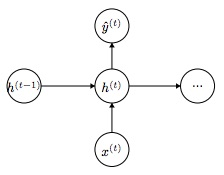
\includegraphics[width=0.7\textwidth]{rnn-timestep}
	\caption{A snapshot of the RNN hidden layer transformation at time step t}
	\label{fig:neural-net}
\end{figure}

In this problem, we are trying to build an RNN to do word prediction, each time step could be occurrence of a particular word. The RNN would output the prediction for the next word given the current input word and the accumulated context within the hidden layer.

\section{Setup}
Similar to the examples from the lecture notes, this problem deals with a single hidden layer RNN. The cost function is again the cross entropy loss function, however now we indicate the time step t at which the error occurred:

$$\vlayer{J}{t}(\theta) = - \sum_{j=1}^{|V|} \slayer{y}{t}{j} log(\slayer{\hat{y}}{t}{j})$$

The errors are summed across all time steps in the sequence to calculate the total loss for that sequence and then the errors for all sequences are summed to calculate the total loss for the data set.

The hidden layer at time step t is calculated as 
$$ \vlayer{h}{t} = \sigma\left(H\vlayer{h}{t-1} + L\vlayer{x}{t}\right)$$

where $\sigma$ is the sigmoid function. The output layer at time step t is calculated as 
$$ \hat{y} = \rho \left(U\vlayer{h}{t}\right)$$
where $\rho$ is the softmax function. The $\hat{y}$ vector is the probabilities the next word, i.e.:
$$P(x_{t+1} = v_j | x_t,\dots,x_1) = \slayer{\hat{y}}{t}{j}$$
$\vlayer{h}{0}$ is a fixed initialization vector. Here, $\vlayer{x}{t}$ is a one hot vector, and thus just "selects" a row from $L$. Thus our dimensions are:

$$H \reals{D_h \times D_h}, L \reals{D_h\times|V|}, U \reals{|V| \times D_h}$$

We can see $L$ contains the representations of the input word, $H$ is the hidden to hidden layer weights matrix, and $U$ is the output weight matrix. $|V|$ is the size of the vocabulary and $D_h$ is the size of the hidden layer.
\section{Understanding Back Propagation Through Time (BPTT)}
Some formulas were presented in the lectures without much justification. We'll go through them here. First we define the overall cost function for a sequence:
$$J = -\frac{1}{T}\sum_{t=1}^{T}\vlayer{J}{t}(\theta) = -\frac{1}{T}\sum_{t=1}^{T}\sum_{j=1}^{|V|}\slayer{y}{t}{j} log(\slayer{y}{t}{j})$$
This is simply the sum of all the costs at each time step. if we want to calculate $\deriv{J}{H}$, we can phrase this as
$$\deriv{J}{H} = \sum_{t=1}^{T} \deriv{\vlayer{J}{t}}{H}$$
Remember H is the same at each time step. So calculating $\deriv{\vlayer{J}{t}}{H}$ is not straight forward. Let's take a look at this network "unrolled" through a few time steps:

\begin{figure}[H]
	\centering
	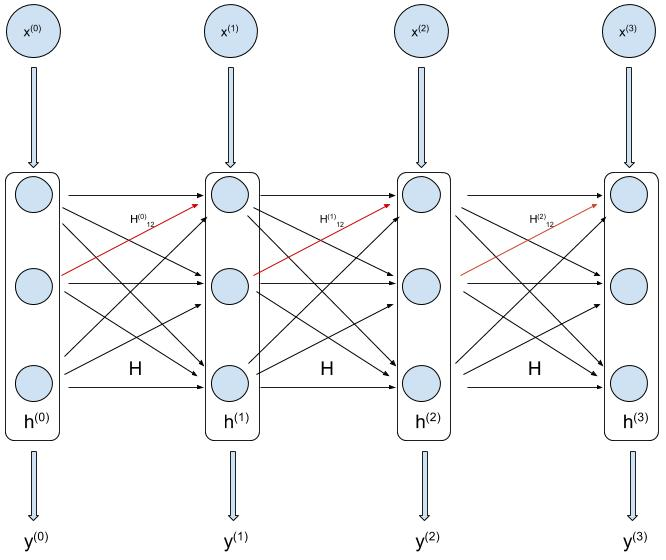
\includegraphics[width=1.0\textwidth]{rnn-unrolled}
	\caption{A RNN across 4 time steps}
	\label{fig:rnn-unrolled}
\end{figure}

Here we see an RNN through 4 time steps. Each time step has an input\vlayer{x}{t}, the current state of the hidden layer\vlayer{h}{t}, and an output vector\vlayer{y}{t} (really \vlayer{\hat{y}}{t}, but here it's y due to limited drawing tool).\vlayer{h}{0} is the initialization vector and each subsequent \vlayer{h}{t} depends on \vlayer{h}{t-1} via the weights matrix $H$. Note $H$ is the \textit{same} weights matrix at each time step!
\paragraph{}
\vlayer{J}{3} here is a function of\vlayer{\hat{y}}{3}. But\vlayer{\hat{y}}{3}is a function of all the previous hidden layers and $H$. The thing to do is think of things element-wise. Let's take a particular weight, $H_{12}$ (highlighted as the red arrow). For clarity, the diagram has labeled each instance of $H_{12}$ separately as \slayer{H}{t}{12}, but again remember it's the same weight at each time step. So to compute how $J$ changes with $H_{12}$, we need to sum how it changes with each particular "instance" of $H_{12}$ in the network:

$$\deriv{\vlayer{J}{3}}{H_{12}} = \sum_{i=0}^{t-1} \deriv{\vlayer{J}{3}}{\slayer{H}{i}{12}}$$
$$ = \deriv{\vlayer{J}{3}}{\vlayer{h}{3}}\cdot\deriv{\vlayer{h}{3}}{H_{12}} + \deriv{\vlayer{J}{3}}{\vlayer{h}{2}}\cdot\deriv{\vlayer{h}{2}}{H_{12}} + \deriv{\vlayer{J}{3}}{\vlayer{h}{1}}\cdot\deriv{\vlayer{h}{1}}{H_{12}}$$

The important thing to see here is the first element of the sum is only considering the impact of \slayer{H}{2}{12},\vlayer{h}{2} is considered as fixed in that element. Similarly, the second term only considers \slayer{H}{1}{12} and the final term only\slayer{H}{0}{12}. Now we can generalize the above formula for $t$ time steps and with respect to each weight $H_{ij}$ represented by the full matrix $H$:

$$\deriv{\vlayer{J}{3}}{H} = \sum_{i=1}^{t} \deriv{\vlayer{J}{t}}{\vlayer{h}{i}}\cdot\deriv{\vlayer{h}{i}}{H}$$
Applying the chain rule:
$$\deriv{\vlayer{J}{3}}{H} = \sum_{i=1}^{t} \deriv{\vlayer{J}{t}}{\vlayer{\hat{y}}{t}}\cdot\deriv{\vlayer{\hat{y}}{t}}{\vlayer{h}{t}}\cdot\deriv{\vlayer{h}{t}}{\vlayer{h}{i}}\cdot\deriv{\vlayer{h}{i}}{H}$$

The difficult thing here to calculate is $\deriv{\vlayer{h}{t}}{\vlayer{h}{i}}$. Via the chain rule we can see that this is simply:

$$\prod_{k=i+1}^{t}\deriv{\vlayer{h}{k}}{\vlayer{h}{k-1}}$$

To calculate $\deriv{\vlayer{h}{k}}{\vlayer{h}{k-1}}$, we can perform some element wise calculations. Note \vlayer{x}{t} as a subscript just means the index of the one hot element:

$$\deriv{\slayer{h}{t}{i}}{\slayer{h}{t-1}{j}} = \deriv{}{\slayer{h}{t-1}{j}}\sigma\left(H\vlayer{h}{t-1} + L\vlayer{x}{t}\right)_{i}$$
$$ = \deriv{}{\slayer{h}{t-1}{j}}\sigma\left(\sum_kH_{ik}\slayer{h}{t-1}{k} + L_{x^{(t)}k}\right)$$
$$ = \sigma'\left(\sum_kH_{ik}\slayer{h}{t-1}{k} + L_{ik}\right) \cdot H_{ij}$$

Let's define the $\sigma'(...)$ term as $\sigma'_i$ for notational convenience. Then in Jacobian matrix form:
\[
\deriv{\vlayer{h}{k}}{\vlayer{h}{k-1}} = 
\begin{bmatrix}
\deriv{\slayer{h}{k}{1}}{\slayer{h}{k-1}{1}}	&	\deriv{\slayer{h}{k}{1}}{\slayer{h}{k-1}{2}}        & \dots & \deriv{\slayer{h}{k}{1}}{\slayer{h}{k-1}{D_h}} \\
\vdots	&	\vdots	&	\ddots	& \vdots \\
\deriv{\slayer{h}{k}{D_h}}{\slayer{h}{k-1}{1}}	&	\deriv{\slayer{h}{k}{D_h}}{\slayer{h}{k-1}{2}}	& \dots & \deriv{\slayer{h}{k}{D_h}}{\slayer{h}{k-1}{D_h}} \\
\end{bmatrix}
\]
\[
\deriv{\vlayer{h}{k}}{\vlayer{h}{k-1}} = 
\begin{bmatrix}
\sigma'_1H_{11}       & \sigma'_1H_{12} & \sigma'_1H_{13} & \dots & \sigma'_1H_{1D_h} \\
\sigma'_2H_{21}       & \sigma'_2H_{22} & \sigma'_2H_{23} & \dots & \sigma'_2H_{2D_h} \\
\vdots	& \vdots	&\vdots	&\ddots	& \vdots \\
\sigma'_{D_h}H_{D_h1}       & \sigma'_{D_h}H_{D_h2} & \sigma'_{D_h}H_{D_h3} & \dots & \sigma'_{D_h}H_{D_hD_h} \\
\end{bmatrix}
\]
$$= diag(\sigma') \cdot H$$

The diag as the leading matrix in a multiplication simply weights the 2nd matrix's rows by the diagonal elements of the first. In later derivations, it will often be useful to phrase this derivative as the inverse Jacobian. In that case we have:

$$\deriv{\vlayer{h}{k}}{\vlayer{h}{k-1}} = H^\top \cdot diag(\sigma')$$

\section{Part a}
Part (a) asks us to show that minimizing the cross entropy loss function from Section 2 will minimize perplexity, given as :
$$ PP(y, \hat{y}) = \frac{1}{\sum_{j=1}^{|V|}\slayer{y}{t}{j}\cdot\slayer{\hat{y}}{t}{j}}$$

Given a correct class k, we have:
$$J(theta) = -log(\slayer{\hat{y}}{t}{k}) , PP(y, \hat{y}) = \frac{1}{\slayer{\hat{y}}{t}{k}} $$
It's clear that as $\hat{y}$ increases, both values monotonically decrease. Thus minimizing the cross entropy loss should minimize perplexity. 

\section{Part b}
Part b asks us to calculate the gradients a time step t, with the previous time steps considered fixed. As before, we'll proceed element wise and then convert the results to vector notation/operations. We'll again change some notation. $U$ and $H$ will be unchanged but we'll again use $a$ and $z$ to refer to layer outputs and inputs, respectively.\vlayer{a}{h,t} and\vlayer{z}{h,t} will refer to the output and input of the hidden layer at time $t$. Similarly, $(x,t)$ and $(o,t)$ superscript will refer to the input and output layer at time $t$.

First we calculate $\deriv{\vlayer{J}{t}}{U}$. As we've seen before, the derivative of the softmax and cross entropy loss combination simply results in a $\hat{y} - y$ vector. We term the input to the final output layer at time t as\vlayer{z}{3,t}
$$\deriv{\vlayer{J}{t}}{U} = \deriv{\vlayer{J}{t}}{\vlayer{z}{3,t}}\cdot\deriv{\vlayer{z}{3,t}}{U} \triangleq\vlayer{\delta}{3,t}\cdot\deriv{\vlayer{z}{3,t}}{U}$$
Element wise for the 2nd term:
$$ \deriv{\slayer{z}{3,t}{i}}{U_{ij}} = \deriv{}{U_{ij}} \sum_{k} U_{ik}\slayer{h}{t}{k}$$
$$ = \slayer{h}{t}{j}$$

In matrix form we have:
\[
\nabla_{U} = 
\begin{bmatrix}
\slayer{\delta}{3,t}{1}\slayer{h}{t}{1}       & \slayer{\delta}{3,t}{1}\slayer{h}{t}{2} & \slayer{\delta}{3,t}{1}\slayer{h}{t}{3} & \dots & \slayer{\delta}{3,t}{1}\slayer{h}{t}{D_h} \\
\slayer{\delta}{3,t}{2}\slayer{h}{t}{1}       & \slayer{\delta}{3,t}{2}\slayer{h}{t}{2} & \slayer{\delta}{3,t}{2}\slayer{h}{t}{3} & \dots & \slayer{\delta}{3,t}{2}\slayer{h}{t}{D_h} \\
\vdots	& \vdots	&\vdots	&\ddots	& \vdots \\
\slayer{\delta}{3,t}{|V|}\slayer{h}{t}{1}       & \slayer{\delta}{3,t}{|V|}\slayer{h}{t}{2} & \slayer{\delta}{3,t}{|V}\slayer{h}{t}{3} & \dots & \slayer{\delta}{3,t}{|V|}\slayer{h}{t}{D_h} \\
\end{bmatrix}
\]
Thus:
\begin{equation} \label{eq:d3,t}
\nabla_U = (\vlayer{\delta}{3,t})(\vlayer{h}{t})^\top
\end{equation}We can check the dimensions and see we end up with $\nabla_U \reals{|V| \times D_h}$, which is correct as it matches the dimensions of $U$.

Next we calculate \deriv{\vlayer{J}{t}}{H}, again element-wise. We define $\vlayer{z}{t,h}$ as the input hidden layer:
$$\deriv{\vlayer{J}{t}}{H_{ij}} = \deriv{\vlayer{J}{t}}{\slayer{z}{t,h}{i}} \deriv{\slayer{z}{h,t}{i}}{H_{ij}}$$
\end{document}